\chapter{Introduction}
\section{High frequency trading system}
\subsection{Evolution of high frequency trading}
Over the last few decades, information technology, including computing speed and memory volume, has made great development. According to this trend, a new class of trading system, which is called high frequency trading (HFT), has appeared to today's financial markets. Generally speaking,  HFT represents a program trading platform that uses powerful computers to transact a great number of orders at very fast speeds. It becomes more and more popular because of some key factors:\\
\begin{itemize}
\item \textbf{Narrowing Spreads}. In 2001, the unit of quoting prices in U.S. Stock exchanges changed from fractions to decimals. so the minimum spread between the bid and ask prices decreased from 1/6th of a dollar (6.25 cents) to one cent. The change of  price unit provides traders better alternatives to seek spread arbitrages, which results in a strong boost in algorithmic trading system.  \\
\item \textbf{Regulation changes}. In 2005, the Securities and Exchange Commission(SEC) passed the Regulation National Market System(Reg.NMS), which improved transparency and competition among different financial markets. Besides, this regulation also required trade orders to be posted nationally instead of at individual exchanges. So traders can be beneficial of profit from small price difference of a security among different exchanges. \\
\end{itemize}

High frequency trading is an extension case of algorithmic trading, which turns over small positions of a security very frequently. The U.S. Securities and Exchanges Commission conclude specific characteristics of HFT:\\

\begin{itemize}
\item Submit some orders and cancel them soon after the submission.
\item Maintain very few or no overnight positions. 
\item Maintain very short time intervals for specific security positions and turn over very frequently of many small positions in one or more financial tools.
\item Utilize complicated and high performance computing program to generate, execute or cancel orders.
\item Make use of individual data from exchanges and servers that belong to co-location provider in order to minimize network or other types of latencies. 
\end{itemize}

According to recent survey(\cite{hft_future}), high frequency trading has taken a great number of share in U.S. and European equity trading volume. As shown in figure \ref{fig.1}, in U.S., the percentage of HFT in equity turnover by volume maintained growth trend overall from year 2005 to 2010. For example, in 2010, HFT occupied 56\% by volume of the entire equity turnover, increased from 21 \% in 2005. 

\begin{figure}[hbtp]
  \begin{center}
    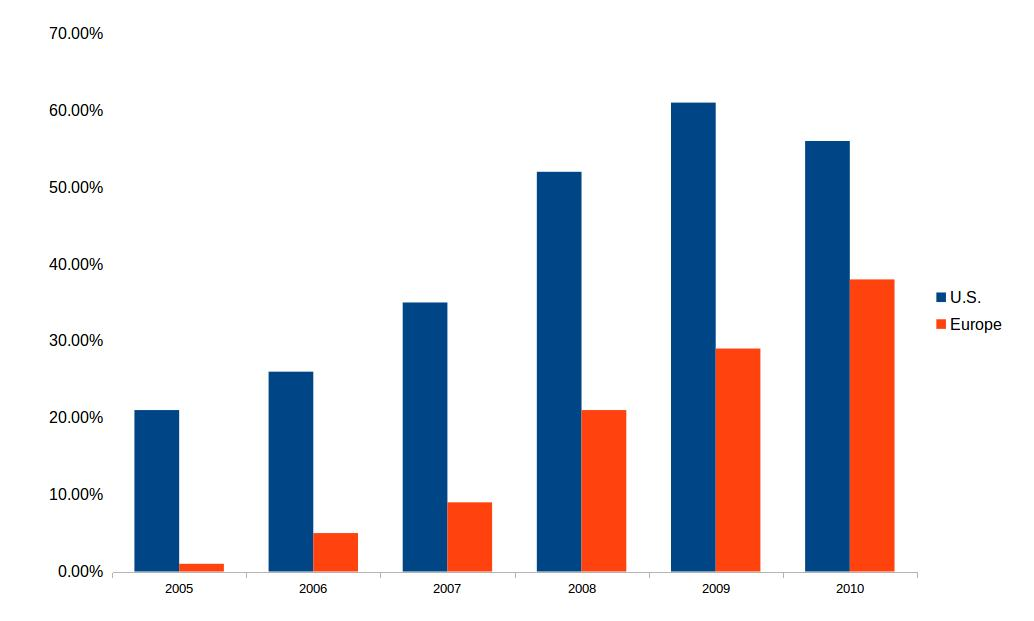
\includegraphics[width=6.5in,height=3.5in]{figures/hft_percentage.jpg}
  \end{center}
\caption{High frequency trading as a \% of equity turnover by volume, U.S. and by value, Europe 2005-2010} \label{fig.1}
\end{figure}

Similar situation happened in Europe. HFT only accounted for 1\% of equity turnover by value in 2005. The percentage surged to 38 \% in 2010, increased from 29 \% just a year ago.
\subsection{High frequency trading strategies}
Generally speaking, there are two main high frequency trading strategies: passive and aggressive trading strategies. Passive strategies uses limit orders which let the brokerage to buy or sell the stocks at a specified level price, while aggressive strategies utilizes market orders to buy or sell the stocks immediately. In the following, we give the description of main types of these two trading strategies. 

For passive HFT strategies, the first widely used method is passive market making. This method allow the market maker to purchase a company's securities and,at the same time, the market maker is also acted as an underwriter of the 
securities in a secondary public offering. Since the market maker can place bids of a security before its publication, the real buyers would have to place their buy orders higher than the market maker's bid price. Therefore the market maker can  benefit from this higher opening. The second method for passive strategies is arbitrage trading. As described by its name, this method makes profit by the price difference of the same or related securities. A simple example is as following: the stock of one company that we called X is trading at \$10 on the New York Stock Exchange(NYSE), while at the same moment it is trading at the price of \$10.05 on the London Stock Exchange(LSE).  Given that a trader can trade the stock on both market with no time lag, he can buy the stock on the NYSE and immediately sell the same shares on the LSE. Obviously, a profit of 5 cents without risk can be earned by him. Those arbitrage opportunity will persist until the specialists on the NYSE or LSE adjust their price to eliminate the price difference.

The main type of aggressive HFT strategies consists of the following two types:
Momentum ignition and order anticipate. The former one is a strategy that a proprietary trading firm buy or sell volumes of orders that will cause the price of underlying security significantly going up or down in the near future. Such quick submission and cancellation of many orders of a stock will trigger other traders' algorithm  to buy or sell the same stock more aggressively. After the trend of price movement is made in the market, the momentum maker will benefit from selling the stock at a higher price or buying the stock at a lower price. However it is very difficult to distinguish between momentum ignition and $\textit{spoof}$, which was defined as illegal according to Dodd Frank Act.  For the order anticipate method, it can be described as a liquidity detection trading which confirms the existence of large institutional buys or sellers in the marketplace and then trade ahead of these buyers or cellers in anticipation that their large orders will move market prices( Securities and Exchange Commission,2014,p.8). The line between this method and another illegal action called \textit{front-running} can be nuanced. The \textit{front-running} is the unethical practice that a stockbroker trades securities in his personal account based on the knowledge of advance knowledge of pending orders from its customers. 

\section{Limit order book dynamics}
According to the above section, we know that under the aggressive strategies situation, it is very likely that the strategy will be deemed as illegal. Therefore choosing passive strategies in high frequency trading is a good idea. Since most transactions in the passive trading strategies are buying and selling the securities at a specific price, limit order books play an indispensable role in this strategy.  
Actually, in today's financial market, more than half of stock exchanges now use a limit order book(LOB) mechanism to facilitate trade(\cite{rosu2009dynamic}).  Some exchanges, such as Helsinki, Hong Kong, Shenzhen, Swiss, Tokyo, Toronto, and
Vancouver Stock Exchanges, now use pure LOBs(\cite{luckock2001statistical}). Some exchanges use hybrid of hybrid LOBs, which include  the New York Stock Ex-change (NYSE), NASDAQ, and the London Stock Exchange
(LSE) \citep{cont2010stochastic}. 

As described above, we can see that LOBs play an important role in financial trading architectures, it is beneficial for both scholars and practitioners to understand dynamics of LOB. The advantages of capturing dynamics of LOBs include: finding optimal opportunity to execute orders\citep{obizhaeva2013optimal}; improving performance of electronic trading algorithms\citep{engle2006measuring}; Obtaining a better understanding of market micro structure for Practitioners\citep{harris2003trading}; Getting a clearer insight into market volatility\citep{kirilenko2015flash}.

In this thesis, we first introduce basic definitions of LOBs, including math definition of bid-ask spread, mid price, bid and ask side depth, spread crossing opportunities and so on. Then we use statistical and data driven methods,especially in the area of machine learning architectures, to model the future arbitrage opportunities of LOBs. We focus on ensemble machine learning algorithms to build our prediction models. As far as we know, there are no evidence shows that these methods were used in LOBs research area. Introduction of ensemble machine learning algorithms will be given in the following section of this chapter and details can be found in chapter ???.  


\section{Ensemble method for classifiers}

In spite of a great amount of research on limit order books, there is only a few literature which utilize machine learning methods for capturing the limit order books. Furthermore, based on our knowledge, there is little evidence that ensemble methods were allied to this topic. In our research, we try to use AdaBoost(Adaptive boosting) method, which was deemed as the best classifier off the shelf\citep{kegl2013return}, and random forest method to predict spread crossing over opportunities of LOBs. 

Generally speaking, an ensemble classifier contains a set of individually trained classifiers(such as neural networks or decision trees) to get better predictive performance by combining the predicting results of each individual classifier. Some past research show that ensemble classifier is generally more accurate than any of the individual classifier which constitutes the ensemble. For example, \cite{hansen1990neural} and \cite{hashem1997optimal} have conducted both theoretical and empirical research which demonstrated that a good ensemble of neural networks are more accurate than its basic classifier. \\

Like other machine learning classifiers, ensemble methods are double edged swords. The main advantage of ensembles is that there is little probability that all classifiers will make the same mistake. Actually, if each error is made by a minority of the classifiers, you can obtain an optimal classification. Besides,ensembles are very likely to reduce the variance of classifiers. Therefore, if the classification algorithms are sensitivity to small changes in the training data, ensemble methods tend to be very helpful.
The disadvantages of ensemble methods are also significant, the biggest might be the lack of interpretation\citep{buhlmann2012bagging}.  A linear combination of individual classifier is much harder to interpret than a single classifier. 

In our research, we utilize two typical ensemble algorithms, AdaBoost and random forest, to train and predict the labeled spread crossing over in a fixed time interval of LOBs. The price spread crossing opportunities can be labeled as ask price lower, bid spread higher and no crossing over in a fixed time horizon. Therefore our problem is a multi-class classification case, the one against one and one against all methods will be introduced to solve the multi-class classification problem. The real time data is divided into two part with the percentage of 9:1, to make a training dataset and testing data set respectively. Besides, features with price, volume and order book arrival intensity of each price level are created, ,so every data sample in training and testing dataset is represented as a vector of features. Moreover, Precision, recall and F1 score  are used to measure the performance of the models, since the existence of arbitrage in a relatively long time interval is rare and our dataset can be treated as an imbalanced data.  

Experiments with real time data from NASDAQ show that the ensemble models built in our paper can not only predict the arbitrage opportunities with high accuracy, but also can improve the prediction performance compared with basic classifiers, such as logistic regression, support vector machine and decision trees. We also design a naive trading strategy in the testing time interval and demonstrate the Profit and Loss (PnL) of our models. The cumulative Pnl curve show that the traders can obtain positive return with zero investment, which indicates that the statistical arbitrages can be found in our models.
\begin{center}
\begin{tikzpicture}[node distance=2cm]
\node (start) [startstop] {Start};
\tikzstyle{io} = [trapezium, trapezium left angle=70, trapezium right angle=110, mimum width=3cm, minimum height=1cm, text width=3cm,text centered, draw=black, fill=blue!30]
\node (in1) [io,below of=start] {Input test\_set[i] features into model};
\node (pro1) [process, below of=in1] {For i= 1 to length(test\_set)};

\node (dec1) [decision, below of=pro1,yshift=-0.5cm] {Predict[i]==1 };
\node (pro2a) [process, right of=dec1, xshift=2cm] {Sell short at bid price,clear the short position  $\Delta_t$ seconds later};
\node (dec2) [decision, below of=dec1, yshift=-2cm] {Predict[i]==-1};
\node (pro2b) [process, right of=dec2, xshift=2cm] {Buy at ask price  Sell at bid price $\Delta_t$ seconds later} ;
\node (pro3) [process, below of=dec2, yshift=-0.5cm] {Take no action} ;
\draw [arrow] (start) --  (in1);
\draw [arrow] (in1) -- (pro1);
\draw [arrow] (pro1) --  (dec1);
\draw [arrow] (dec1) -- node[anchor=south] {yes} (pro2a);
\draw [arrow] (dec2) -- node[anchor=south] {yes} (pro2b);
\draw [arrow] (dec1) -- node [anchor=east] {no} (dec2);
\draw [arrow] (dec2) -- node[anchor=east] {no} (pro3);
\end{tikzpicture}
\end{center}
\section{Purpose of the dissertation}

